\section
[$M^X/M/1$ Queue Length Distribution]
{$\mathbf{M^X/M/1}$ Queue Length Distribution}
\label{sec:batch-arrivals}


\subsection*{Theory and Exercises}

\Opensolutionfile{hint}
\Opensolutionfile{ans}

In Sections~\ref{sec:mxm1-queue:-expected} and~\ref{sec:mg1} we established the Pollackzek-Khintchine formula for the waiting times of the $M^X/M/1$ queue and $M/G/1$ queue, respectively. To compute more difficult performance measures, for instance the loss
probability $\P{L>n}$, we need expressions for the stationary distribution of the number of jobs in the system $p(n)=\P{L=n}$.   Here we present a numerical, recursive, scheme to compute the stationary distribution of the number of items in an $M^X/M/1$ queue. 

To find the distribution $p(n)$, which is equal to $\pi(n)$ by PASTA,
we turn to level-crossing arguments. However, the arguments that lead
to the level-crossing equation~\eqref{eq:15} need to be generalized.  To
see this, we consider an example.  If $L(t)=3$, the system contains
$3$ items (but not necessarily $3$ jobs.)  Since the server serves
single items, down-crossings of level $n=3$ occur in single
units. However, due to the batch arrivals, when a job arrives it
typically brings multiple items to the queue. For instance, suppose
that $L(A_k-) = 3$, i.e., job $k$ sees 3 items in the system at its
arrival epoch.  If $B_k = 20$, then  right
after the arrival of job $k$ the system contains 23 items, that is, $L(A_k)=3+20=23$. In this
case, at the arrival of job $k$, all levels between states $3$ and
$23$ are crossed.  

The left panel in Figure~\ref{fig:levelcrossing} demonstrates the up- and downcrossings in more general terms.  Level $n$ can be up-crossed
from below from many states, in fact from any level $m, 0\leq m <n$. However,
it can only be down-crossed from state $n+1$.


% As a consequence, it is not
% necessarily the case that $|A(n,t) - D(n,t)| \leq 1$ for all $t$, as
% was the case for queueing systems in which jobs arrive as single
% units. We need to generalize this inequality.

\begin{figure}[ht]
  \centering
\begin{tikzpicture}[scale=1,
    %Define standard arrow tip
    >=stealth',
    %Define style for boxes
    circ/.style={
      circle, 
      draw=black,
      thick,
      minimum size=1.cm,
      inner sep=0pt,
      text centered
    },
    % Define arrow style
    pil/.style={
           ->,
           thick,
           shorten <=2pt,
           shorten >=2pt}
]

\draw[dashed, thick] node at (5,-1.5) [below]  {level $n$} 
(5,-1.5) -- (5,3);

\node[circ] (n-2) {$n-2$};
\node[circ, right=of n-2] (n-1) {$n-1$}
edge[loop below, thick]  node[midway, fill=white] {$\lambda f(0)$} (n-1); 
\node[circ, right=of n-1] (n) {$ n $}
   edge[pil,<-, bend left=45] node[below] {$\lambda f(1)$} (n-1.south east);
\node[circ, right=of n] (n+1) {$n+1$}
   edge[pil,bend left=45] node[midway, fill=white] {$\mu$} (n.south east);
\node[above=of n+1] (inf) {}
   edge[pil, <-, bend right=45] node[midway, fill=white] {$\lambda G(0)$} (n.north east)
   edge[pil, <-, bend right=45] node[midway, fill=white] {$\lambda G(1)$} (n-1.north east)
   edge[pil, <-, bend right=45] node[midway, fill=white] {$\lambda G(2$} (n-2.north east)
;
\end{tikzpicture}
%  \begin{tabular}
%    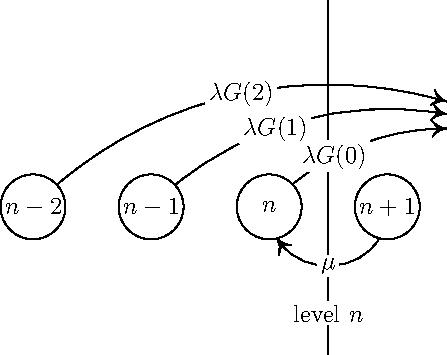
\includegraphics[scale=0.9]{mxm1_2}
%&
%    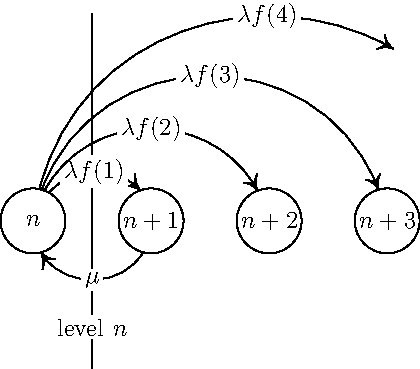
\includegraphics[scale=0.9]{mxm1_1}
%  \end{tabular}
  \caption{Level crossing of level $n$.  Observe
    that when the system is in state $n-2$, the arrival of any batch
    larger than $2$ ensures that level $n$ is crossed from below.  The
    rate at which such events happen is $\lambda G(2)$.
    Similarly, in state $n-1$ the arrival of any batch larger than one
    item ensures that level $n$ is crossed, and this occurs with rate
    $\lambda G(1)$, and so on.  
% In the right panel we see all the
%     transitions from state $n$ (the state in which the system contains
%     $n$ units of work) such that level $n$ is crossed from below.
%     Clearly, with rate $\lambda \P{X=1} = \lambda f(1)$ jobs
%     containing one item arrive; if such an event occurs, the system
%     moves from $n$ items to $n+1$ items.  With with rate
%     $\lambda f(2)$ jobs with two items work arrive, so that the system
%     contains $n+2$ units of work after the arrival of such jobs, and
%     so on. Level $n$ is crossed from above, i.e., the system moves
%     from state $n+1$ to $n$, when a unit of work is processed, which
%     happens at rate $\mu$. To relate the left and the right panel,
%     observe in the right panel that any `arrow' from state $n$ to the
%     right crosses level $n$. All these rates added together are such
%     that
%     $\lambda \sum_{i=1}^\infty f(i) = \lambda \P{B\geq 1} = \lambda
%     \P{B>0} = \lambda G(0)$.
%     A similar reasoning applied to state $n-1$ shows that only the
%     arrows such that $\lambda \sum_{i=2}^\infty f(i) = \lambda G(1)$
%     cross level $n$, and so on. 
  }
  \label{fig:levelcrossing}
\end{figure}

As always with level-crossing arguments, we turn to counting how often
level $n$ is upcrossed and downcrossed as a function of time. The
downcrossing rate is easy; it is exactly the same as for the $M/M/1$
queue. Thus, from Eq.~\eqref{eq:22}, 
\begin{equation}
\frac{D(n,t)}t = \frac{D(n,t)}{Y(n+1,t)}\frac{Y(n+1,t)}t
\end{equation}
which, as $t\to\infty$, converges to the downcrossing rate
\begin{equation}
\mu(n+1) p(n+1) = \mu \pi(n+1),
\end{equation}
where we use that $\mu(n+1) = \mu$ by the memoryless property of the
service times and PASTA to see that $\pi(n+1)=p(n+1)$.  Observe that
this part was easy because there is just one way (i.e., there is just
one arrow from right to left in Figure~\ref{fig:levelcrossing}) to
downcross level $n$, namely from $n+1$ to $n$. 

Counting upcrossings requires quite some more work. Observe that
$\1{L(A_k-)\leq n}=1$ only when the $k$th job sees~$n$ or less items in the system, and
$\1{L(A_k) > n}=1$ only when after the $k$th arrival the system contains more than $n$ items. Thus, $\1{L(A_k-) \leq n}\1{ L(A_k)>n}=1$ only when the $k$th arrival generates an upcrossing of level~$n$. 
%  Hence
% \begin{equation*}
%   \sum_{k=1}^{A(t)} \1{L(A_k-) \leq n}\,\1{L(A_k)>n}
% \end{equation*}
% counts all upcrossings  of level $n$ up to time $t$.


From Figure~\ref{fig:levelcrossing} we see that an upcrossing can be decomposed into:
\begin{equation*}
  \begin{split}
&\1{L(A_k-) \leq n}\1{L(A_k)>n}  \\
&=  \1{L(A_k-) =n}\, \1{B_k >0} + \1{L(A_k-) =n-1}\1{ B_k >1} +\cdots + \1{L(A_k-) =0}\1{B_k > n} \\
&= \sum_{m=0}^n \1{L(A_k-) =m}\1{B_k > n-m}.
  \end{split}
\end{equation*}
In other words, paths that upcross level $n$ require that any job that
sees $m$ ($m\leq n$) in the system upon arrival must bring a batch larger
than $n-m$ items.

Next, define 
\begin{equation*}
  A(m,n,t) = \sum_{k=1}^{A(t)}\1{L(A_k-) = m}\1{B_k > n-m}
\end{equation*}
as the number of jobs up to time $t$ that see $m$ in the system upon
arrival and have batch size larger than $n-m$. 

\begin{exercise}
   Show that $A(n, n,t) = A(n,t)$, where $A(n,t)$ is defined by Eq.~\ref{eq:19}.
\begin{solution}
 $A(n,n,t)$ counts all jobs up to time $t$ that see $n$ items
    and bring at least $n-n+1=1$ unit of work. As each job brings at
    least 1 item, $A(n,n,t)$ counts all jobs that see $n$ items at
    arrival.
\end{solution}
\end{exercise}

As in Section~\ref{sec:level-cross-balance}, we are primarily interested in  long-run averages. For this purpose, observe that we can write
\begin{equation}\label{eq:16}
  \frac{A(m,n,t)}t =   \frac{A(t)}t \frac{A(m,t)}{A(t)}\frac{A(m,n,t)}{A(m,t)}.
\end{equation}
By the assumptions of Section~\ref{sec:poisson-arrivals-see},  $A(t)/t\to\lambda$ and $A(m,t)/A(t)\to\pi(m)$.  Now, provided the limit exists, we define
\begin{equation}\label{eq:1332}
\lim_{t\to\infty} \frac{A(m,n,t)}{A(m,t)} = 
\lim_{t\to\infty} \frac{\sum_{k=1}^{A(t)}\1{L(A_k-) = m, B_k > n-m}}
{\sum_{k=1}^{A(t)}\1{L(A_k-) = m}}=\P{B>n-m\given L(A-)=m},
\end{equation}
where the random variable $L(A-)$   denotes the number in the system seen by an arbitrary arrival.

\begin{exercise}
Show that $\P{B>n-m\given L(A-)=m}=\P{B>n-m}$
\begin{solution}
  \begin{hint}
    Realize that $B$ and $L(A-)$ are assumed to be independent.
  \end{hint}
\begin{equation*}
  \begin{split}
\P{B>n-m\given L(A-)=m} &=
\frac{\P{B>n-m,L(A-)=m}}{\P{L(A-)=m}}\\
&=\frac{\P{B>n-m}\P{L(A-)=m}}{\P{L(A-)=m}} = \P{B>n-m}.
  \end{split}
\end{equation*}
\end{solution}
\end{exercise}

By the above exercise,
\begin{equation*}
\lim_{t\to\infty} \frac{A(m,n,t)}{A(n,t)} = \P{B>n-m} = G(n-m).
\end{equation*} 
By combining the above and making the usual assumptions about the
existence of all limits involved we find
\begin{equation*}
\lim_{t\to\infty}   \frac{A(m,n,t)}t = \lambda \pi(m) G(n-m).
\end{equation*}

\begin{exercise}
Provide an interpretation of the above result in terms of a thinned Poisson arrival process.
\begin{solution}
Eq.~(\ref{eq:16}) has the interpretation that the rate at which
level $n$ is crossed from below from state $m$ is equal the rate at
which jobs arrive times the fraction of jobs that see $m$ jobs in the
system times the fraction of jobs with batch size larger than $n-m$.
Observe that the stream of jobs with batch size larger than $n-m$
is a Poisson process thinned at rate $G(n-m)$. 
\end{solution}
\end{exercise}


The last step is to relate the up- and downcrossing rates.  Clearly, $\sum_{m=0}^n A(m,n,t)$ is  the total number of times level $n$ is upcrossed up to time~$t$. By level crossing,
 \begin{equation*}
 \sum_{m=0}^n A(m,n,t) \approx  D(n,t). 
\end{equation*}
Thus, taking the limit $t\to\infty$ in this equation, we conclude that
\begin{equation}\label{eq:42}
\lambda  \sum_{m=0}^n G(n-m) \pi(m) = \mu \pi(n+1).
\end{equation}

\begin{exercise}
  Show that Eq.~(\ref{eq:42}) reduces to $\mu p(n+1)=\lambda p(n)$ for the $M/M/1$ case.
  \begin{solution}
    The left hand side of Eq.~(\ref{eq:42}) is identical, so we only
    have to concentrate on the right hand side. In the $M/M/1$ queue,
    all batches have size $1$. Thus, $\P{B=1} = f(1)=1$ and $f(k)=0$
    for $k\neq 1$. Thus, $G(0)=1$ and $G(1)=G(2)=\cdots = 0$. Thus,
    $\sum_{m=0}^n G(n-m) p(m) = G(0)p(n)=p(n)$.
  \end{solution}
\end{exercise}

\begin{exercise}\label{ex:13}
With $\alpha = \lambda/\mu$,  show that \emph{unnormalized} state probabilities are given by
\begin{align*}
\pi(0) & = 1 &
  \pi(1) &= \alpha \\
  \pi(2) &= \alpha^2 + \alpha G(1), &
  \pi(3) &= \alpha[ \alpha^2 + 2 \alpha G(1)) + G(2)].
\end{align*}
We leave the rest to the computer to continue with this.
\begin{hint}
For $n=1$, we have
$\mu \pi(1) = \lambda \pi(0)=\lambda$. Use that $G(0)=1$.
\end{hint}
\begin{solution}
\begin{equation*}
  \begin{split}
  \pi(1) &= \alpha \\
  \pi(2) &= \alpha G(0) \pi(1) + \alpha G(1) \pi(0) =\alpha(\alpha+ G(1)) = \alpha^2 + \alpha G(1), \\
  \pi(3) 
&= \alpha[G(0) \pi(2) + G(1) \pi(1) + G(2) \pi(0)]  = \alpha[ \alpha^2 + 2 \alpha G(1)) + G(2)],
  \end{split}
\end{equation*}
\end{solution}  
\end{exercise}

It is left to find the normalization constant.  As this recursion does
not lead to a closed form expression for $p(n)$, such as
Eq.~\eqref{eq:23}, we need to use a criterion to stop this iterative
procedure. Finding general conditions on when to stop is not directly
easy, but a pragmatic approach is to simply stop at some (large)
number $N$ such that $p(k)\ll p(0)$ for $k>N$ and is steadily decreasing. (An interesting question, why should it decrease monotonically after some, large, $N$?)
Then take $G=\sum_{i=0}^N \pi(i)$ as the normalization
constant, so that $\pi(0)=1/G$, $\pi(1)=\alpha/G$, and so on.
While this is a practical approach, getting formal bounds on a proper size of $N$ requires more work than we can do here.

Now that we have the state probabilities, we can compute the \emph{excess probability}
\begin{equation}
  \P{L> n } = \sum_{i=n+1}^\infty \pi(i).
\end{equation}
This performance measure is  of interest in inventory systems or---recall the supermarket example discussed in the Introduction---when there are costs associated with the occurence of long queues. 

An interesting extension is to consider a queueing process with batch
services, i.e., the $M/M^Y/1$ queue. Construction a recursion for the
steady-state probabilities $p(n)$ for this case is not hard, in fact,
mostly analogous to Eq.~(\ref{eq:42}).  However, solving the recursion
appears to be quite a bit harder; we will not discuss this further here

\begin{exercise}
  Why is Eq.~\eqref{eq:39}, i.e., $\pi(n)=\delta(n)$, not true for the
  $M^X/M/1$ batch queue?
\begin{solution}
 Because arrivals do not occur in single units, but in batches.
\end{solution}
\end{exercise}

Let us use  recursion Eq.~(\ref{eq:42}) for $\pi(n)$ to
 derive an expression for the expected number of units of work $\E L$
 in the system.
\begin{exercise}
 Show that
\begin{equation}\label{eq:67}
  \mu \E L =\mu \sum_{n=0}^\infty n \pi(n) = \lambda \frac{\E{B^2}}2  + \lambda \E B \E L +\lambda \frac{\E B}2,
\end{equation}
\begin{hint}
Substitute the
  recursion, and carry on with the algebra. We urge the reader to try
  it, its good (necessary) practice.  Use also the results of the
  exercises of Section~\ref{sec:mxm1-queue:-expected}.  
\end{hint}
\begin{solution}
  We use that $\mu \pi(n) =\lambda \sum_{i=0}^{n-1} \pi(i) G(n-1-i)$
  and the results of the exercises of
  Section~\ref{sec:mxm1-queue:-expected} to see that
\begin{align*}
  \mu \E L
  &=\sum_{n=0}^\infty n\, \mu \pi(n), \quad \text{now substitute for $\mu \pi(n)$ the above recursion}, \\
& =\lambda \sum_{n=0}^\infty n \sum_{i=0}^{n-1} \pi(i) G(n-1-i) 
  =\lambda \sum_{n=0}^\infty n \sum_{i=0}^\infty 1\{i<n\} \pi(i) G(n-1-i) \\
& =\lambda \sum_{i=0}^\infty \pi(i) \sum_{n=0}^\infty 1\{i<n\} n G(n-1-i) 
  =\lambda \sum_{i=0}^\infty \pi(i) \sum_{n=i+1}^\infty n G(n-1-i) \\
& =\lambda \sum_{i=0}^\infty \pi(i) \sum_{n=0}^\infty (n+i+1) G(n) 
  =\lambda \sum_{i=0}^\infty \pi(i) \left[\sum_{n=0}^\infty n G(n) +(i+1) \sum_{n=0}^\infty G(n)\right]  \\
  &=\lambda \sum_{i=0}^\infty \pi(i)\sum_{n=0}^\infty n G(n) +\lambda  \E B \sum_{i=0}^\infty \pi(i) (i+1)  \\ 
  &=\lambda \sum_{i=0}^\infty \pi(i) \frac{\E B^2 -\E B}2  + \lambda \E B (\E L +1)  \\ 
  &= \lambda \frac{\E B^2 -\E B}2  + \lambda \E B \E L +\lambda \E B \\
  &= \lambda \frac{\E B^2 }2  + \lambda \E B \E L +\lambda \frac{\E B}2,
\end{align*}
\end{solution}
\end{exercise}

With this we can check a result of Section~\ref{sec:mxm1-queue:-expected}.  
\begin{exercise}
  Use Eq.~(\ref{eq:67}) and the definition for
  $\rho=\lambda \E B/\mu$ to show that
\begin{equation*}
(1- \rho) \E L = \frac{\lambda}\mu \frac{\E{B^2}}2 + \frac\rho2.
\end{equation*}
\begin{hint}
Divide both sides by $\mu$.
\end{hint}
\begin{solution}
Dividing both sides by $\mu$ and using that $\lambda \E B/\mu = \rho$, 
\begin{equation*}
  \E L = \frac{\lambda}{\mu}  \frac{\E B^2 }2 + \rho \E L + \frac\rho2.
\end{equation*}
\end{solution}
\end{exercise}



\begin{exercise}
  Implement the recursion~(\ref{eq:42}) in a computer program for the
  case $f(1)=f(2)=f(3)=1/3$ (recall $\P{B=k} =f_k$). Take $\lambda =1$
  and $\mu = 3$.  
  \begin{hint}
This is an important problem, it helps to check (numerically)
    the algebraic results we have been deriving up to
    now. Implementing the recursion is not hard, just try and see how
    far you get.
  \end{hint}
  \begin{solution}
The recursion for $n$ becomes 
\begin{equation*}
\pi(n) = \frac \lambda \mu \sum_{i=0}^{n-1} \pi(n-1-i)G(i).
\end{equation*}
Since $G(i) =0$ for $i\geq 3$ we rewrite this to 
\begin{equation*}
  \pi(n) = \frac\lambda \mu \sum_{i=0}^{\min(\{n-1,l\}} \pi(n-1-i)G(i),
\end{equation*}
where $l=3$. 

In python this reads:

\begin{pyverbatim}
p[n] = labda / mu * sum(p[n - 1 - i] * G[i] for i in range(min(n, l)))
\end{pyverbatim}

The following code carries out the recursion for the $M/M/1$ queue and compares the result to the \emph{unnormalized} probabilities $(\lambda/\mu)^n$ (unnormalized means that I do  not multiply with $1-\rho$). Thus, we can test the code right away. 

\begin{pyconsole}
import numpy as np

l = 1 # M/M/1 has batch size 1
f = np.ones(l + 1) / l # f[0] =1, f[1] = 1 
f[0] = 0 # set f[0] = 0
F = np.cumsum(f) # distribution 
G = np.ones_like(F) - F # survivor function

labda = 1
mu = 3
num = 30
p = np.ones(num)

for n in range(1, num):
    p[n] = labda / mu * sum(p[n - 1 - i] * G[i] for i in range(min(n, l)))
    print(n, p[n], (labda / mu)**n)

\end{pyconsole}
The test is convincing.

\begin{pyconsole}
l = 3
f = np.ones(l + 1) / l
f[0] = 0
F = np.cumsum(f)
G = np.ones_like(F) - F
num = 30
p = np.ones(num)
for n in range(1, num):
    p[n] = labda / mu * sum(p[n - 1 - i] * G[i] for i in range(min(n, l)))
    print(n, p[n])

\end{pyconsole}
Stopping at 30 seems ok. The last step is normalize.
\begin{pyconsole}
p /= p.sum()  # normalize
for n in range(1, num):  # print normalized results
    print(n, p[n])

\end{pyconsole}

Now that we have the probabilities we can do all experiments we like. 
\begin{pyconsole}
EL = sum(n*p[n] for n in range(len(p)))
EL 
\end{pyconsole}

It is of interest to compare this result to the equation above
Eq.~(\ref{eq:43}).


\begin{pyconsole}
EB = sum(k*fk for k,fk in enumerate(f))
EB2 = sum(k*k*fk for k,fk in enumerate(f))
EB2
rho=labda*EB/mu
RHS = labda/mu*EB2/2 + rho/2
EL=RHS/(1-rho)
EL
\end{pyconsole}

So, after all, stopping at 30 seems not quite ok: there is a slight
difference between the two expectations. Let's run the recursion up to
100, and see what we get then.

\begin{pyconsole}
num = 100
p = np.ones(num)

for n in range(1, num):
    p[n] = labda / mu * sum(p[n - 1 - i] * G[i] for i in range(min(n, l)))

p /= p.sum()  # normalize
EL = sum(n*p[n] for n in range(len(p)))
print(EL)
\end{pyconsole}
This does the job.

As a last step, I want to check Eq.~(\ref{eq:43}). In fact, I spent at least one hour to
get Eq.~(\ref{eq:43}) correct. Now I can also numerically check it.

\begin{pyconsole}
VB = EB2 - EB*EB
C2 = VB/EB/EB
EL = (1+C2)/2*rho/(1-rho)*EB + rho/(1-rho)/2
EL
\end{pyconsole}
The results agree. 
\end{solution}
\end{exercise}


\begin{exercise}(Finite queueing systems) We consider the $M^X/M/1/K$
queue, i.e., a batch queue in which at most $K$ jobs fit into the
system. When customers can be blocked, it is necessary to specify an
acceptance, or equivalently a rejection, policy. Three common rules are
\begin{enumerate}
\item Complete rejection: if a batch does not fit entirely into the system, it will be rejected completely.
\item Partial acceptance: accept whatever fits of a batch, and reject the rest.
\item Complete acceptance: accept all batches that arrive when the
  system contains $K$ or less jobs, and reject otherwise.
\end{enumerate}
Derive a set of recursions, analogous to Eq.~(\ref{eq:42}), to compute
$\pi(n)$ for these three different acceptance rules.  
\begin{hint}
This
  exercise tests your creativity and modeling skills, it is not
  analytically difficult.  The best approach to problems like this is
  to try some simple cases first. For instance, consider the case with
  batch sizes of $1$ first, then batches of sizes $1$ or $2$, and so
  on. If system contains $K$ jobs, which batches can be accepted? If
  the system contains $K-3$, say, which batch sizes can be accepted,
  which will be refused, under which acceptance policy? 
\end{hint}
\begin{solution}
  Let's first deal with complete rejection. Suppose a batch of size
  $k$ arrives when the system contains $n$ jobs. When $k+n \leq K$,
  the batch can be accepted since the entire batch will fit into the
  queue.  When, however, $k+n> K$, the batch has to be rejected. 

  Now consider an imaginary line between states with $n$ and $n+1$
  jobs in the system. This imaginary line separates the state space
  into two disjoint part: one part with states $0, 1, \ldots, n$ and
  the other part with states $n+1, n+2, \ldots, K$. We call this
  imaginary line `level $n$'.  We call an `upcrossing' a transition
  from some state $m\leq n$ to a state $l> n$. Likewise, a `downcrossing'  of level~$n$ is a transition from some state $l> n$ to some state $m\leq n$.

  If the system contains $n$ jobs,  level $n$ is
  crossed from below with rate $\lambda \pi(n) \P{B \leq K-n}$.  More generally,
  when the system is in state $m\leq n$, we need a batch of at least
  $n+1-m$ to cross level~$n$. Moreover, any batch larger than $K-m$
  gets rejected. Thus, when the system contains $m \leq n $ jobs, the
  rate at which level $n$ is crossed from below is
  \begin{equation*}
  \lambda \pi(m) \P{n+1-m\leq B \leq K-m}  = \lambda \pi(m)
  [G(n-m)-G(K-m)],
  \end{equation*}
where we use that
\begin{align*}
\P{n+1-m\leq B \leq K-m} 
&= \P{B \leq K-m} - \P{B \leq n-m}  \\
&= \P{B > n-m} - \P{B > K-m} \\
&= G(n-m)-G(K-m).
\end{align*}

  Since the server serves only single items, level $n$ can only be
  crossed from above from state $n+1$. This happens at rate $\mu p(n+1)$. With PASTA this is equal to $\mu \pi(n+1)$.

  Finally, since on the long run the number of up- and crossings must
  be the same, the up- and downcrossing rates must match. This implies
  that the balance equations becomes
  \begin{equation*}
    \mu \pi(n+1) = \lambda \sum_{m=0}^n \pi(m)   [G(n-m)-G(K-m)],
  \end{equation*}
  for $n=0,\ldots, K-1$. 

  Before we continue with the other acceptance rules, it is important
  to check this result.  In general, off-by-one errors are easily, and
  commonly, made, so we need to test the above on simple cases. 
  \begin{itemize}
  \item  If $K\to \infty$, then $G(K-m)=\P{B>K-m}\to 0$, so we get our earlier result. 
  \item Take $n=K$. Then $G(n-m)-G(K-m)=0$ for all $m$. Then the right hand side is 0, as it should.
  \item Taken $n=0$ and $K=1$, then $\mu \pi(1)= \lambda \pi(0)$. This also makes sense. 
  \item Take $n$ much smaller than $K$. If the batch size is maximally
    $2$, then for small $n$ the entire batch must fit. Let's see if
    this holds in the above formula. If $n$ much smaller than $K$,
    then also $m$ is much smaller than $K$ (since in the right hand
    size, $m\leq n$. But then $G(K-m) \leq G(2) = 0$, as it
    should. (Observe that $G$ is a decreasing function of its argument;
    its a survival function.)
  \end{itemize}

  The complete-acceptance policy is actually quite simple. As any
  batch will be accepted when $n\leq K$, the queue length is not
  bounded.  Only when the number of jobs in the system is larger than
  $K$, we do not accept jobs. 
  \begin{equation*}
    \mu \pi(n+1) = 
    \begin{cases}
      \lambda \sum_{m=0}^n \pi(m) G(n-m), & \text{ for } n\leq K,\\
      \lambda \sum_{m=0}^K \pi(m) G(n-m), & \text{ for } n> K.
    \end{cases}
  \end{equation*}





  For the partial acceptance case, any job is accepted, but the system
  only admits whatever fits.  As level $n\in {0,1,...,K-1}$ is still upcrossed by any batch of size at least $n-m$ when the system is in state $m$, the formula for the upcrossing rate is identical to the case without this acceptance policy. Moreover, nothing changes to the formula for the downcrossing rate. Hence, 
  \begin{equation*}
    \mu \pi(n+1) = \lambda \sum_{m=0}^n \pi(m) G(n-m), 
  \end{equation*}
  for $n=0,1,\ldots, K-1$. 
\end{solution}
\end{exercise}




\Closesolutionfile{hint}
\Closesolutionfile{ans}

\opt{solutionfiles}{
\subsection*{Hints}
\input{hint}
\subsection*{Solutions}
\input{ans}
}

%\clearpage

%%% Local Variables:
%%% mode: latex
%%% TeX-master: "../book"
%%% End:
